\documentclass{article}
\usepackage[utf8]{inputenc}
\usepackage{polski}
\usepackage{graphicx}
\usepackage{amsmath}

\title{\textbf{Issac Newton}}
\author{Damian Lechański \break Rafał Motyka}

\begin{document}
\maketitle

\centerline{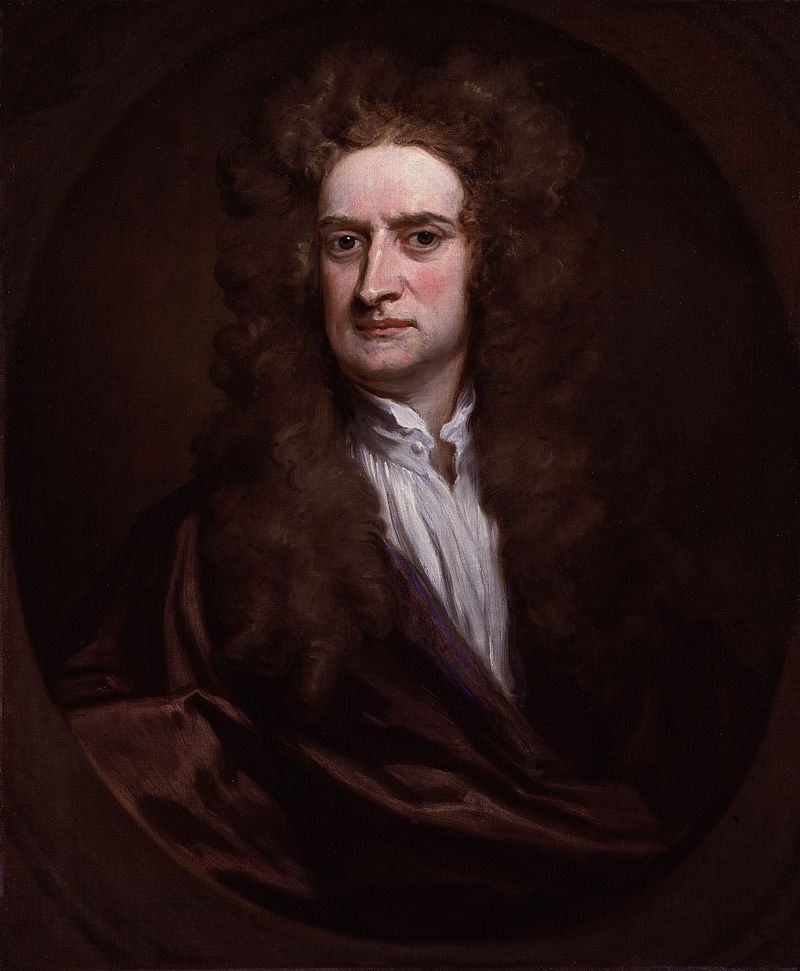
\includegraphics[width=120mm,scale=0.6]{images/Newton.jpg}}



\newpage
\section{Wstęp}
Urodził się 25 grudnia 1642/4 stycznia 1643 w Woolsthorpe-by-Colsterworth, zm. 20 marca/31 marca 1727 w Kensington. (Daty nowego i starego porządku)\newline Angielski fizyk, matematyk, astronom, filozof, historyk, badacz Biblii i alchemik. Odkrywca trzech zasad dynamiki.

\section{Życiorys}
\subsection{Młodość}
\textbf{Newton} urodził się w Woolsthorpe koło Colsterworth, w hrabstwie Lincolnshire, trzy miesiące po śmierci swego ojca, również Isaaca. Dwa lata później jego matka Hannah wyszła ponownie za mąż za Barnabasa Smitha i pozostawiła syna pod opieką babki.\newline
\textbf{Newton} pobierał nauki w Grantham Grammar School, gdzie uczono głównie łaciny, a także w nieco mniejszym stopniu greki i hebrajskiego. W 1661 r. rozpoczął edukację w Trinity College w Cambridge, gdzie wcześniej studiował jego wuj William Ayscough. W tamtych czasach programy nauczania w College’u oparte były na dziełach Arystotelesa, ale Newton wolał poznawać dzieła współczesnych uczonych, takich jak Kartezjusz, Galileusz, Kopernik i Kepler. W 1665 odkrył twierdzenie o dwumianie i rozpoczął pracę nad teorią matematyczną znaną obecnie jako rachunek różniczkowy i całkowy. Wkrótce po tym jak Newton uzyskał stopień naukowy w 1665 r., uniwersytet został zamknięty z powodu zarazy. Przez następne dwa lata \textbf{Newton} pracował w zaciszu domowym nad rachunkiem różniczkowym i całkowym, a także optyką i grawitacją.\newline
Legenda głosi, że \textbf{Newton} siedział pod jabłonią, gdy spadające na jego głowę jabłko uświadomiło mu, że upadek ciał na Ziemię i ruch ciał niebieskich są powodowane tą samą siłą – grawitacją. Historia ta jest wyolbrzymieniem opowieści samego \textbf{Newtona}, który jakoby siedząc pewnego dnia przed oknem w swoim domu obserwował spadające z drzewa jabłka. Jednak obecnie uważa się, że nawet ta historia jest fałszywa i została wymyślona przez Newtona pod koniec jego życia, który w ten sposób chciał pokazać, że potrafi czerpać inspirację z codziennych zdarzeń. Pisarz William Stukeley opisał w swoich Memoirs of Sir Isaac Newton’s Life rozmowę z Isaakiem Newtonem w Kensington 15 kwietnia 1726 r., w której Newton powiedział mu, że „kiedy pierwszy raz przyszło mu na myśl pojęcie grawitacji, było to przy okazji widoku spadającego jabłka, kiedy siedział w nastroju kontemplacyjnym. Zadał sobie wtedy pytanie, dlaczego jabłko zawsze spada pionowo w kierunku ziemi. Dlaczego nie podąża na boki albo ku górze, ale zawsze w kierunku centrum Ziemi”. W podobny sposób wyraził się Voltaire w swoim dziele zatytułowanym Essay on Epic Poetry (1727 r.).


\section{Dokonania}
\subsection{Symbol Newtona}
Symbol Newtona, współczynnik dwumianowy (dwumienny) Newtona – funkcja dwóch argumentów całkowitych nieujemnych, zdefiniowana jako:

\begin{equation}
	{{n}\choose{k}}=\frac{n!}{k!(n-k)!} \quad \mathrm{dla} \quad 0\le k \leq n
\end{equation}

Symbol Newtona można równoważnie wyrazić wzorem rekurencyjnym:

\begin{equation}
{{n}\choose{k}}=
\begin{cases}
1 \quad \quad \quad \quad \quad \quad \,\,\, \mathrm{dla} \quad k=0 \quad \mathrm{lub} \quad k=n\\
{{n-1}\choose{k-1}}+{{n-1}\choose{k}}\quad \mathrm{dla} \quad 0 < k < n
\end{cases}
\end{equation}


\newpage
\tableofcontents
\end{document}
